\documentclass[dvipdfmx, 
				border = {5pt, 5pt, 5pt, 5pt}]{standalone}	% borderで余白をあける

\usepackage{tikz}	% ティクス
\usetikzlibrary{intersections, math, patterns}
% intersections .. 交点の座標を求めるため
% math .. 計算を行う
% patterns .. 領域をパターンで塗りつぶすため

\begin{document}

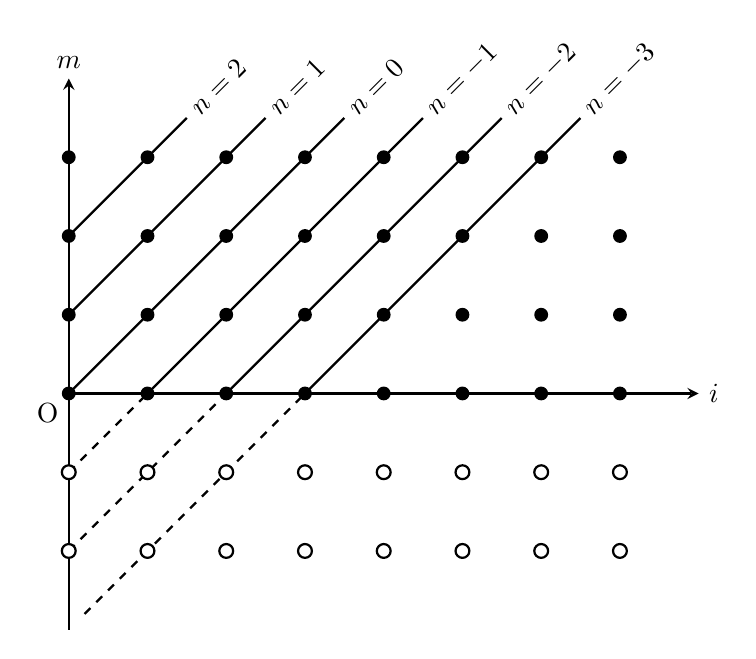
\begin{tikzpicture}[domain = -1.5:4, samples = 100, thick]	% sampleじゃなくてsamples
  \draw (0, 0) node[below left]{O};		% 原点

  % 斜線を引く
   %\fill [top color = white, bottom color = white, middle color = purple]
	% plot[sample = 100, domain = 0:4] (\x, {\x / 2 + 2})
	%(4, 4)--(4, 0)--(1, 0)--(0, 1) --(0, 2) -- (4, 4);

  % 斜線を引く
  % \fill [pattern = north east lines, very thin]		% 薄くしたいんだが
  %	% plot[sample = 100, domain = 0:4] (\x, {\x / 2 + 2})
  %	(4, 4)--(4, 0)--(1, 0)--(0, 1) --(0, 2) -- (4, 4);

  % 軸の描画
  \draw [thick, -stealth] (0, 0)--(8, 0) node[right] {$i$};			% x軸
  \draw [thick, -stealth] (0, -3)--(0, 4) node[above] {$m$};		% y軸

  % 点線
  % 縦
  % \foreach \i in {1, 2, 3, 4, 5, 6, 7}
  %   \draw[thin, dashed] (\i, -3)--(\i, 5);
  % 横
  % \foreach \i in {-2, -1, 0, 1, 2, 3, 4}
  %   \draw[thin, dashed] (0, \i)--(8, \i);
  

  % 直線の描画
  \draw[domain = 0:1.5] plot(\x, {\x+2})
	node [right, rotate=45, fill=white] {$n=2$};

  \draw[domain = 0:2.5] plot(\x, {\x+1})
	node [right, rotate=45, fill=white] {$n=1$};

  \draw[domain = 0:3.5] plot(\x, {\x})
	node [right, rotate=45, fill=white] {$n=0$};

  \draw[domain = 1:4.5] plot(\x, {\x-1})
	node [right, rotate=45, fill=white] {$n=-1$};

  \draw[domain = 2:5.5] plot(\x, {\x-2})
	node [right, rotate=45, fill=white] {$n=-2$};
  
  \draw[domain = 3:6.5] plot(\x, {\x-3})
	node [right, rotate=45, fill=white] {$n=-3$};

  \draw[dashed] (0, -1)--(1, 0);
  \draw[dashed] (0, -2)--(2, 0);
  \draw[dashed] (0.2, -2.8)--(3, 0);
  
  
  % 黒点
  \foreach \i in {0, 1, 2, 3, 4, 5, 6, 7}
    \foreach \j in {0, 1, 2, 3}
      \fill (\i, \j) circle [radius=2.5pt];

  % 白丸
  \foreach \i in {0, 1, 2, 3, 4, 5, 6, 7}
    \foreach \j in {-2, -1}
      \draw[fill=white] (\i, \j) circle (2.5pt);
  
      
  % \draw [thin, dashed] (1, -0.8)--(1, 4.5)
  %	node [left, fill = white, inner sep = 0pt] at(0.8, 4) {$x_1 = \frac{k}{\alpha}$};
  

  % 関数の描画
  % \draw [domain = -1.2:2] plot(\x, {-\x + 1}) 
  % 	node [right, fill = white, inner sep = 0pt]  at(2.1, -0.9) {$x_1 + x_2 = 1$};

  
  % 領域D
  % \draw (2.1, 1.5) node [fill = white] {$D$};

  % 座標
  % \node [below left] at(1, 0) {1};
  % \node [left] at(0, 1) {1}; 
  % \node [above left] at(0, 2) {2};		% left above ではだめ

\end{tikzpicture}

\end{document}
